\documentclass[twocolumn, a4paper]{article}
\usepackage{graphicx}
\usepackage{amsmath}
\begin{document}
\title{$\Gamma$-function}
\author{Wikipedia}
\maketitle
\begin{abstract}
In mathematics, the gamma function (represented by $\Gamma$, the capital letter gamma from the Greek alphabet) is one commonly used extension of the factorial function to complex numbers.
\end{abstract}
\section{Introduction}
\begin{equation}\label{eq-def}
	\Gamma(z) = \int_0^\infty x^{z-1} e^{-x}\,dx, \ \qquad \Re(z) > 0\ .
\end{equation}

Here is a reference to an equation \eqref{eq-def}.

\begin{figure} [b]
	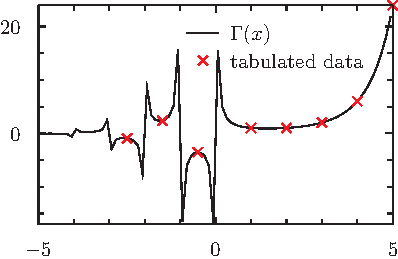
\includegraphics{gamma_pyx.pdf}
\end{figure}
\end{document} 
